\documentclass[a4paper,14pt,russian]{extreport}
 
\usepackage{extsizes}
\usepackage{cmap} % для кодировки шрифтов в pdf
\usepackage[T2A]{fontenc}
\usepackage[utf8]{inputenc}
\usepackage[russian]{babel}
%\usepackage{pscyr} % набор красивых шрифтов
 
\usepackage[dvips]{graphicx} % для вставки картинок
\graphicspath{{images/}}
\usepackage{amssymb,amsfonts,amsmath,amsthm} % математические дополнения от АМС
\usepackage{indentfirst} % отделять первую строку раздела абзацным отступом тоже
\usepackage[usenames,dvipsnames]{color} % названия цветов
\usepackage{makecell}
\usepackage{multirow} % улучшенное форматирование таблиц
\usepackage{ulem} % подчеркивания
 
\linespread{1.3} % полуторный интервал
\renewcommand{\rmdefault}{ftm} % Times New Roman
\frenchspacing

\usepackage{fancyhdr}
\pagestyle{fancy}
\fancyhf{}
\fancyhead[R]{\thepage}
\fancyheadoffset{0mm}
\fancyfootoffset{0mm}
\setlength{\headheight}{17pt}
\renewcommand{\headrulewidth}{0pt}
\renewcommand{\footrulewidth}{0pt}
\fancypagestyle{plain}{ 
    \fancyhf{}
    \rhead{\thepage}}
\setcounter{page}{1} % начать нумерацию страниц с №1

\usepackage[tableposition=top]{caption}
\usepackage{subcaption}
\DeclareCaptionLabelFormat{gostfigure}{Рисунок #2}
\DeclareCaptionLabelFormat{gosttable}{Таблица #2}
\DeclareCaptionLabelSeparator{gost}{~---~}
\captionsetup{labelsep=gost}
\captionsetup[figure]{labelformat=gostfigure}
\captionsetup[table]{labelformat=gosttable}
\renewcommand{\thesubfigure}{\asbuk{subfigure}}

\usepackage{titlesec}
\titleformat{\chapter}[display]
    {\filcenter}
    {\MakeUppercase{\chaptertitlename} \thechapter}
    {8pt}
    {\bfseries}{}
\titleformat{\section}
    {\normalsize\bfseries}
    {\thesection}
    {1em}{}
\titleformat{\subsection}
    {\normalsize\bfseries}
    {\thesubsection}
    {1em}{}
     
% Настройка вертикальных и горизонтальных отступов
\titlespacing*{\chapter}{0pt}{-30pt}{8pt}
\titlespacing*{\section}{\parindent}{*4}{*4}
\titlespacing*{\subsection}{\parindent}{*4}{*4}

\usepackage{geometry}
\geometry{left=3cm}
\geometry{right=1.5cm}
\geometry{top=2.4cm}
\geometry{bottom=2.4cm}

\usepackage{enumitem}
\makeatletter
    \AddEnumerateCounter{\asbuk}{\@asbuk}{м)}
\makeatother
\setlist{nolistsep}
\renewcommand{\labelitemi}{-}
\renewcommand{\labelenumi}{\asbuk{enumi})}
\renewcommand{\labelenumii}{\arabic{enumii})}

\usepackage{tocloft}
\renewcommand{\cfttoctitlefont}{\hspace{0.38\textwidth} \bfseries\MakeUppercase}
\renewcommand{\cftbeforetoctitleskip}{-1em}
\renewcommand{\cftaftertoctitle}{\mbox{}\hfill \\ \mbox{}\hfill{\footnotesize Стр.}\vspace{-2.5em}}
\renewcommand{\cftchapfont}{\normalsize\bfseries \MakeUppercase{\chaptername} }
\renewcommand{\cftsecfont}{\hspace{31pt}}
\renewcommand{\cftsubsecfont}{\hspace{11pt}}
\renewcommand{\cftbeforechapskip}{1em}
\renewcommand{\cftparskip}{-1mm}
\renewcommand{\cftdotsep}{1}
\setcounter{tocdepth}{2} % задать глубину оглавления — до subsection включительно

\newcommand{\empline}{\mbox{}\newline}
\newcommand{\likechapterheading}[1]{ 
    \begin{center}
    \textbf{\MakeUppercase{#1}}
    \end{center}
    \empline}
    
\makeatletter
    \renewcommand{\@dotsep}{2}
    \newcommand{\l@likechapter}[2]{{\bfseries\@dottedtocline{0}{0pt}{0pt}{#1}{#2}}}
\makeatother
\newcommand{\likechapter}[1]{    
    \likechapterheading{#1}    
    \addcontentsline{toc}{likechapter}{\MakeUppercase{#1}}}

\usepackage[square,numbers,sort&compress]{natbib}
\renewcommand{\bibnumfmt}[1]{#1.\hfill} % нумерация источников в самом списке — через точку
\renewcommand{\bibsection}{\likechapter{Список литературы}} % заголовок специального раздела
\setlength{\bibsep}{0pt}

\parindent = 1cm

\begin{document}
% НАЧАЛО ТИТУЛЬНОГО ЛИСТА
\begin{center}
\hfill \break
\large{МИНОБРНАУКИ РОССИИ}\\
\footnotesize{ГОСУДАРСТВЕННЫЙ УНИВЕРСИТЕТ}\\ 
\small{\textbf{«МОСКОВСКИЙ ФИЗИКО-ТЕХНИЧЕСКИЙ ИНТСИТУТ»}}\\
\hfill \break
\normalsize{Факультет управления и прикладной математики}\\
 \hfill \break
\normalsize{Кафедра системного программирования}\\
\hfill\break
\hfill \break
\hfill \break
\hfill \break
\large{Исследование возможностей распараллеливания алгоритмов разрешения ограничений на GPU}\\
\hfill \break
\hfill \break
\hfill \break
\normalsize{Магистерская диссертация\\
\hfill \break
Направление  010100 Математика\\
\hfill \break
Магистерская программа    Вещественный, комплексный и функциональный анализ}\\
\hfill \break
\hfill \break
\end{center}
 
\normalsize{ \hspace{28pt} Допущено к защите в ГЭК  27.05.2015} \hfill \break
\hfill \break
 
\normalsize{ 
\begin{tabular}{cccc}
Зав.кафедрой & \underline{\hspace{3cm}} &  д.физ.-мат.н.,  проф. & Е.М. Семёнов \\\\
Обучающийся & \underline{\hspace{3cm}} & &С.М. Петров \\\\
Руководитель & \underline{\hspace{3cm}}& д.физ.-мат.н., проф.&  Т.Я. Азизов \\\\
\end{tabular}
}\\
\hfill \break
\hfill \break
\begin{center} Долгопрудный 2017 \end{center}
\thispagestyle{empty} % выключаем отображение номера для этой страницы
 
% КОНЕЦ ТИТУЛЬНОГО ЛИСТА
 
\newpage
     
    \tableofcontents % Вывод содержания
\newpage
 
\newpage
\chapter{Введение}
\section{Актуальность}
Данная работа является приклакладным исследованием в области целочисленного программирования, которая относится к более широкой области задач разрешения ограничений. Так как многие важные задачи сводятся к задачам разрешения ограничений (constraint satisfaction problem), им уделяется немало внимания \cite{dechter}, \cite{freuder}, \cite{tsang}. Суть таких задач состоит в нахождении значений переменных, удовлетворяющих заданным ограничениям. 
\par
В общем случае проблема существования решений задачи разрешения ограничений может быть алгоритмически неразрешимой или NP-полной. Программирование в ограничениях широко использует методы целочисленного программирования. Задача существования целочисленного решения системы является NP-полной, поэтому требует больших вычислительных затрат. Таким образом для реальных задач необходимо проделывать очень большой объем вычислений, что не позволяет расширить довольно ограниченный круг задач, для решения которых используются известные методы целочисленного программирования. Актуальность и трудность проблематики делают целочисленное программирование одним из перспективных и интересных направлений в математическом программировании \cite{karmanov}\cite {balinski}.
\par
Использование подходов и алгоритмов теории разрешения ограничений позволяет решать многие прикладные задачи в разработке программного обеспечения, такие как планирование \cite{kautz} и теория расписаний \cite{barnier}, задачи проектирования экспертных систем и систем поддержки принятия решений \cite{saraev}, обработка изображений \cite{montanari}, задачи тестирований интегральных схем \cite{hooker}, формальная верификация и статический анализ. В свою очередь статический анализ широко используется в верификации свойств ПО, которое требует высокой надёжности, например в области медицины, ядерной физики или авиации.
\par
Среди подходов формальной верификации существуют методы построения тестов с помощью символического выполнения (symbolic execution). Такие методы используют символическое описание проходимого во время выполнения теста пути по коду программы (или формальных проверяемых спецификаций) в виде набора предикатов. Это описание позволяет выбирать новые тестовые ситуации так, чтобы они покрывали другие пути и строить тесты с помощью техник разрешения ограничений \cite{gotlieb}, \cite{boyapati}. 
\par 
В литературе можно найти несколько хороших обзоров с описанием методов решения задач разрешения ограничений, включая (Kumar, 1992) cite{kumar}, (Dechter, Frost, 1999) \cite{dechter_frost}, (Bartak, 2001) \cite{bartak}, \cite{meseguer}, \cite{miguel}, а также статьи в энциклопедических сборниках (Dechter, 1992) \cite{dechter_networks}, \cite{hower} и (Mackworth, 1992) \cite{mackworth}.
\par 
Более подробную информацию по теме разрешения ограничений можно найти в монографиях \cite{apt}, \cite{dechter}, \cite{fruehwirth}, \cite{marriott}, \cite{rossi}, \cite{hentenryck}, \cite{hentenryck_michel_deville}, \cite{hentenryck_opl}, \cite{hentenryck_michel}. 
\par 
Линейные неравенства имеют большое самостоятельное значение, поскольку многие математические модели представляются в виде таких систем. Особый интерес линейные неравенства стали представлять в связи с созданием математической экономики \cite{kantorovich} и линейного программирования в середине XX века. Многие модели экономики имеют вид систем линейных неравенств или задач линейного программирования, которые можно считать частным случаем систем линейных неравенств. Основная задача линейного программирования - это нахождение экстремумов линейных фукнций при множестве линейных ограничений. Нас интересует подраздел линейного программирования - целочисленное линейное программирование (integer linear programming, ILP), в котором на все или некоторые переменные дополнительно накладывается ограничение целочисленности. Простейший метод решения задачи целочисленного программирования — сведение её к задаче линейного программирования с проверкой результата на целочисленность.
\par
Задача линейного программирования может быть записана в виде:
$$\max \vec c^T \vec x$$
$$A\vec x \leq \vec b$$, где $\vec c, \vec x \in \mathbb{R}^n, \vec b \in \mathbb{R}^m, A \in \mathbb{R}^{m\times n}$

\section{Постановка задачи}

Расчет сложных хаотических систем вроде погоды, симуляции взаимодействий элементарных частиц в физике, моделирование на нано-уровне, data mining, криптографии очень требовательны к аппаратным ресурсам. При выполнении данных операций используют параллельные вычисления, распределяя нагрузку между ресурсами CPU и процессорами компьютеров кластера.
\par 
GPU имеет тысячи более энергоэффективных ядер, созданных для выполнения нескольких задач одновременно. Представляется актуальным использовать возможности GPU для задачи разрешения ограничений. Таким образом направление вычислений эволюционирует от «централизованной обработки данных» на центральном процессоре до «совместной обработки» на CPU и GPU. Всё чаще GPU применяется для решения вычислительных задач, выходящих за рамки первоначального предназначения этих устройств. В связи с чем в работе исследуются возможности графических карт применительно к задаче целочисленного программирования. 
\par
Технология GPGPU (general-purpose computing for graphics processing units) позволила увеличить на несколько порядков вычислительные возможности компьютеров, пропорционально уменьшив затраты на программное обеспечение. Она позволяет использовать ресурсы видеокарт для неграфических вычислений. Основным производителем видеокарт с аппаратной поддержкой GPGPU является NVIDIA с комплексом CUDA, которая обеспечила рост популярности GPGPU за счёт упрощения процесса создания программ, использующих возможности GPU. Ещё одной популярной реализацией техники GPGPU является OpenCL (open computing language) - фреймворк для написания программ на различных графических и центральных процессорах. Далее в работе рассматривается технология Cuda.
\par
В работе подробно рассматривается один из способов решения системы линейных неравенств общего вида Branch-and-Cut. А точнее находится случайное целочисленное решение системы или констатируется, что целочисленных решений системы не существует.  
\par 
Цель работы - реализация алгоритма Branch-and-Cut с использованием подходов массивного параллелизма и возможностей Nvidia CUDA. Для достижения цели необходимо решить ряд подзадач. При составлении плана использовался план разработки ПО, представленный в \cite{mcconnell}: 
\begin{itemize}
\item[•] Изучить предмет исследования - методы решения задач целочисленного программирования.
\item[•] Изучить инструмент исследования - технология Cuda.
\item[•] Выработать требования к входным данным и результатам.
\item[•] Реализовать алгоритм branch-and-Cut последовательно на CPU.
\item[•] Исследовать алгоритм на наиболее часто повторяющиеся вычисления.
\item[•] Исследовать возможности распараллеливания найденных участков на GPU.
\item[•] Создание параллельного алгоритма Branch-and-Cut, учитывая особенности Cuda.
\item[•] Детальное проектирование алгоритма.
\item[•] Кодирование, отладка и оптимизация.
\item[•] Тестирования.
\item[•] Интерпретация результатов.
\end{itemize}

\section{Обзор существующих решений}
К методам целочисленного линейного программирования относят:
\begin{itemize}
\item[•] метод отсечений (например, метод Гомори);
\item[•] приближённый метод (прямой алгоритм, предложенный Р.Д.Юнгом и Ф.Гловером)
\item[•] метод ветвей и границ (branch-and-bound);
\item[•] комбинированные методы (branch-and-cut);
\item[•] использование абсолютной унимодулярности матрицы (сильно ограничивает множество решаемых систем уравнений);
\item[•] графический метод (если задача содержит две переменные);
\item[•] эвристики:
\begin{itemize}
\item табу-поиск - tabu-search \cite{glover};
\item алгоритм восхождение на вершину - hill climbing \cite{russell};
\item алгоритм имитации отжига \cite{kirkpatrick};
\item оперативная оптимизация поиска;
\item муравьиный алгоритм \cite{colorni};
\item нейронная сеть Хопфилда \cite{lau};
\end{itemize}
\end{itemize}
\par
Недостатком эвристических методов является то, что если алгоритм не может найти решение, то невозможно определить, нет решения или есть, но алгоритм не смог его найти. 
\par

\chapter{Методика решения задачи}
В данной работе рассматривается алгоритм Branch-and-Cut. Во-первых, он не подразумевает ограничения по входным матрицам. 
\section{Branch-and-Cut алгоритм}
Branch-and-Cut - это метод комбинаторной оптимизации для решения целочисленных задач линейного программирования, то есть таких задач, решение которых целочисленно. Техника метода использует решение системы линейных неравенств без наложения ограничения целочисленности. Когда получено оптимальное решение, которое содержит не целочисленное значение одной из целевых переменных, может добавляться отсечение в виде линейного неравенства, которое исключает данное нецелочисленное значение, но включает все возможные целочисленные. После этого решается новая задача линейного программирования, строится новое отсечение и т.д., пока либо не получится оптимальное решение, либо не будет выявлена несовместность условий получившейся задачи линейного программирования. 
\par
Branch-and-Cut алгоритм включает в себя Branch-and-Bound с использованием отсечений, чтобы сузить область поиска решений. В свою очередь Branch-and-Bound основывается на симплекс-методе, который подробно обсуждается в следующем параграфе. Делим задачу на несколько (как правило, две) подзадач и применяем симплекс-метод к получившимся двум.

\begin{enumerate}
\item[1.]
Добавить исходную задачу в множество $L$ - множество активных задач.
\item[2.]
Инициализировать $x^* = \null$ и $v^* = -\infty$
\item[3.]
Пока список $L$ не пуст и не найдено целочисленное решение:
\begin{enumerate}
\item[а)] выбираем проблемы и исключаем её из списка $L$;
\item[б)] решаем выбранную проблему симплекс методом;
\item[в)] если решения нет, то возвращаемся к 3., обозначим значение функции $v$; 
\item[г)] если  $v \le v^*$, то возвращаемся к 3.;
\item[д)] если решение целочисленное, то $v^* \leftarrow v$, $x^* \leftarrow x$ и возвращаемся к 3.;
\item[е)] по желанию добавляем отсечения или отсечение;
\item[;)] ветвимся, создаём на основе решения предыдущей задачи новые(как правило, две) и возвращаемся к 3.;
\end{enumerate}
\item[3.] return найденное решение.
\end{enumerate}
 
\par
До сих пор остаётся открытым вопрос о стратегии ветвления: в какой последовательности генерировать дочерние вершины и какую из дробных координат выбирать для генерации неравенств. К сожалению, здесь мало теоретических результатов и для выбора хорошей стратегии опираютс яна интуицию и вычислительный эксперимент. К хорошим результатам, например, приводит выбор для ветвления вершины с максимальным значением верхней оценки. А для выбора дробной координаты считается разумным выбор той из них, которая приводит к максимальному уменьшению верхней оценки целевой функции. 
\par
Вопрос о наилучшем способе выбора переменной ветвления или последовательности решения конкретных задач в настоящее время не решен. Ветвиться можно несколькими способами. Некоторые из них реализуют ветвление по переменной, т.е. выбирается переменная $x_i$ с нецелочисленным значением $a_i$ и создаются две задачи, каждая из которых является добавлением к предыдущей ограничения $x_i\leqslant \lfloor a_i \rfloor$ и $x_i\geqslant \lceil a_i \rceil$. Например:
\begin{itemize}
\item[•] выбирается переменная наиболее близкая по значению к 0.5;
\item[•] сохраняются треки каждой из переменных и выбирается та, изменение которой, возможно наибольшее;
\item[•] каждая переменная проверяется на наибольшее влияние на целевую функцию, то при ветвлении по которой, фукнция изменится максимально.
\end{itemize}
\par

\par
Многие задачи комбинаторной оптимизации могут быть представлены как смешанные целочисленные задачи линейного программирования. В этом случае применимы branch-and-cut методы, которые по сути есть комбинация метода отсечения и branch-and-bound алгоритма. Эти методы используют решения некоторой последовательности упрощённых целочиселнных задач. Метод отсечений приближает решение к целочисленному, а branch-and-bound делит задачу на несколько других. 
\par

\par
Также branch-and-cut используется для решения задачи линейного упорядочивания (linear ordering problem), максимального отсечения (maximum cut), планирования (scheduling), о рюкзаке (packing), нахождения максимального планарного подграфа и др.
\par

\section{Симплекс-метод}
Симплекс-метод - это алгоритм решения оптимизационной задачи линейного программирования, путём перебора вершин выпуклого многогранника в многомерном пространстве.
\par
Термин симплекс-метод был предложен Моцкиным и Данцигом. Поясним происхождение этого термина. 
\par
{\bf Определение.} Пусть $p_0,p_1,...,p_t \in \mathbb{R}^n$: векторы $q_1=p_1-p_o,q_2=p_2-p_0,...,q_t=p_t-p_0$ линейно независимы. Множество Conv{$p_o,p_1,...,p_t$} называется $t$-мерным симплексом. 
\par 
$n$-мерный симплекс можно описать как множество решений системы, состоящей из $n+1$ неравенства. И наоборот, система неравенств определяет некоторый $n$-мерный симплекс. Таким образом, симплекс-метод можно описать как движение от одного симплекса к соседнему. 
\par
{\bf Определение.} Вектор $p$ лексикографически положителен $p \succ 0$, если его первая отличная от нуля компонента положительна. Вектор $q$ лексикограически больше вектора $p$ ($q \succ p$), если $q-p \succ 0$.

\section{Метод отсечений}
Пусть имеется оптимальное решение задачи линейного программирования, полученной из задачи цеолчисленного линейного программирования отбрасыванием требования целочисленности. Пусть также решение не является полностью целочисленным. Тогда добавим отсечение в виде линейного неравенства, которое исключает данное нецелочисленное значение, но включает все возможные целочисленные. После этого решается новая задача линейного программирования, строится новое отсечение и т.д., пока либо не получится оптимальное решение, либо не будет выявлена несовместность условий получившейся задачи линейного программирования. 
\par 
В общем случае метод представляет собой сиситематическое введение дополнительных ограничений с целью сведения исходной допустимой области к выпуклой оболочке её одпустимых целочисленных точек.
\par
Метод отсечений для решения целочисленных задач а также способ построеня отсечений, гарантирующий конечность процедуры, был впервые предложен Гомори (1963, опубликован в 1958). К сожалению, предложенные им отсечения не были эффективными и медленно сходились, поэтому идея отсечений не рассматривалась много лет. Развитие теории многогранников привели к тому, что метод отсечений вновь привлёк внимание в 1980-х и широко используется в настоящее время. Наиболее известно применение branch-and-cut алгоритма в задаче коммивояжёра (traveling salesman problem). Такой подход оптимален в большинстве случаев по сравнению с другими методами. 
\par
Применение только отсечений не является эффективным методом решения оптимизационных задач. А branch-and-bound алгоритм может быть усовершенствован использованием отсечений, так как они существенно уменьшают размер получаемого дерева.
\par
Отсечениями называют линейные неравенства, которые удовлетворяются целочисленными решениями задачи линейного программирования, но могут нарушаться решениями общей задачи оптимизации.
\par
Так как оптимальное решение после правильного отсечения не является допустимым решением новой задачи линоейного программирования, но является её двойственным допустимым решением, то для решения новой задачи выгоднее использовать двойственный симплекс-метод. Кроме того, так как правильное отсечение явлется неравенством, то удобнее использовать столбцовую форму записи и считать, что ограничения исходной задачи заданы в форме неравенств. (с 119, В.Н.Шевченко и Н.Ю.Золотых).

\section{Допущения используемого метода}
Для этого используется алгоритм, который минимизирует функцию на дискретном множестве, описанном линейными неравенствами и состоящем из целых значений. Но для существующей задачи нет надобности минимизировать, поэтому алгоритм завершается, как только находится первое целочисленное решение. А целевая функция может быть любой. 
\par
Изначально данный алгоритм предназначался для нахождения оптимального решения и поэтому находятся все целочисленные решения. Для целевой задачи дипломной работы достаточно нахождение одного целочисленного решения и поэтому приведённый ниже алгоритм не является полным. 
\par
Как известно различные процессоры могут по-разному производить арифметические операции над переменными типа float или double. Такая же ситуация состоит и с разницей между GPU и CPU. Также необходимо учесть, что математика с исопльзование переменных с плавающей точкой не является сочетательной. Т.е. может быть так, что $(A+B)+C\neq A+(B+C)$. При распараллеливании, потенциально меняется порядок вычислений. В свзяи со всеми этими особенностями необходимо дополнительно проверять сходятся ли результаты различных реализаций на GPU и CPU. 
\par

\begin{enumerate}
\item[1.]
Добавить исходную задачу в множество $L$ - множество активных задач.
\item[2.]
Пока список $L$ не пуст и не найдено целочисленное решение:
\begin{enumerate}
\item[а)] выбираем проблемы и исключаем её из списка $L$;
\item[б)] решаем выбранную проблему симплекс методом;
\item[в)] если решения нет, то возвращаемся к пункту a), иначе проверяем решение на целочисленность;
\item[г)] если решение целочисленное, переходим к 4;
\item[д)] по желанию добавляем отсечения или отсечение;
\item[е)] ветвимся, создаём на основе решения предыдущей задачи новые(как правило, две) и возвращаемся к началу пункта;
\end{enumerate}
\item[3.] return найденное решение.
\end{enumerate}

\section{Описание возможных методов}
Так как симплекс-метод играет ключевую роль в алгоритме Branch-and-Cut, начнём возможные реализации алгоритма именно с этой части.  
\par
При программной реализации алгоритмов линейного программирования одной из возникающих проблем является накопление ошибок округления. 
\par
В первую очередь реализуем весь алгоритм на CPU - то есть последовательно. Первый вопрос, на который следует ответить, - с какими элементами матрицы мы будем работать. Так как используемый симплекс-метод нецелочисленный, может возникнуть проблема округления чисел, что приведёт к неправильному решению даже самых простых задач. Поэтому для большей точности элемент представляем в виде дроби, то есть двух целых чисел. В остальном реализация на CPU была однозначной. Она состоит из трёх частей: поиск строки, поиск столбца, модернизация матрицы:
\begin{enumerate}
\item[1.] Поиск строки - pivot\_row:
  \begin{enumerate}
  \item[а)] ищем первый отрицательный элемент, кроме нулевого, в нулевом столбце;
  \item[б)] если его нет, завершаем алгоритм.
  \end{enumerate}
\item[2.] Поиск столбца:
  \begin{enumerate}
  \item[а)] не считая нулевого элемента, ищем отрицательные элементы в pivot\_row и сохраняем колонну, которой принадлежит этот элемент и нормированную по модулю данного элемента, в некотором временном множестве $P$;
  \item[б)] выбираем наименьшую колонну из множества $P$ - pivot\_col.
  \end{enumerate}
\item[3.] Модернизация матрицы - применяем гауссовы преобразования таким образом, pivot\_row обнулилась, кроме элемента, соответствующего pivot\_col. После преобразований этот элемент должен быть равен -1.
\end{enumerate}
\par
После этого приступаем к алгоритму симплекса на GPU. Первый вопрос, который возникает при подходе к симплекс-методу на GPU, - где хранить матрицу и каких размеров она может быть. 
\par
Мы можем хранить матрицу в памяти графической карты, тем самым избегая постоянного копирования, но тогда поиск pivot\_row и pivot\_col проводя также на GPU. Это недостаток, так как такие задачи плохо распараллеливаются на GPU. 
\par
И как ещё один вариант, мы храним матрицу в памяти центрального процессора и каждый раз копируем из памяти CPU в GPU и наоборот. Графические карты поддерживают как синхронное, так и асинхронное копирование.  Основным достоинством асинхронного копирования является то, что оно позволяет параллельное исполнение ядра (kernel), то есть мы имеем возможность обрабатывать уже скопированные данные во время копирования остальных данных. Но такое копирование медленнее синхронного и может оперировать только с закреплённой памятью. 
\par
В итоге мы имеем три возможные идеи, как реализовать параллельный алгоритм. Каждая идея имеет как свои плюсы, так и недостатки, поэтому в работе я реализовала все три алгоритма. Обобщим теоретические рассуждения в двух таблицах, содержащих достоинства каждого из подходов:
\par
\begin{tabbing}
\hspace{0.5\textwidth} \= \hspace{0.5\textwidth} \kill
{\bf алгоритм с абсолютной реализацией} \> {\bf алгоритм с частичной реализацией} \\ 
{\bf на GPU:} \> {\bf на GPU:} \\
$\cdot$ нет необходимости копировать  \> $\cdot$ плохо распараллеливается на GPU  \\
большие объёмы данных из памяти  \> функция поиска pivot\_row и \\
CPU в память GPU и наоборот \> pivot\_col, так как требуют лишних  \\
 \> затрат для синхронизации алгоритма \\
\end{tabbing}
 
\begin{tabbing}
\hspace{0.5\textwidth} \= \hspace{0.5\textwidth} \kill
{\bf использования синхронного копиро-} \> {\bf использование асинхронного копиро-} \\
{\bf вания} \> {\bf вания} \\
$\cdot$ быстрее \> $\cdot$ параллельная обработка уже скопи- \\
$\cdot$ сильно выигрывает при копирова- \> рованных данных\\
нии маленьких объёмов памяти \>  
\end{tabbing}
\par
При прочих равных условиях преобразования таблицы, количество итераций, 
совершаемых действий и значения ячеек внутри таблицы на каждой итерации не зависит от реализации алгоритма. 

\chapter{Практическая реализация}  
язык программирования, технология CUDA, компилятор, количество строчек кода ))

\section{Сравнение GPU и CPU} 
\cite{poletaev} Рост частот универсальных процессоров упёрся в физические ограничения и высокое энергопотребление, и увеличение их производительности всё чаще происходит за счёт размещения нескольких ядер в одном чипе. Продаваемые сейчас процессоры чаще всего содержат лишь четыре ядра и они предназначены для обычных приложений. И они используют MIMD-архитектуру – множественный поток команд и данных. Каждое ядро работает отдельно от остальных, исполняя разные инструкции для разных процессов. 
\par
В видеочипах NVIDIA, например, основной блок – это мультипроцессор с восемью-десятью ядрами и сотнями ALU в целом, несколькими тысячами регистров и небольшим количеством разделяемой общей памяти. Кроме того, видеокарта содержит быструю глобальную память с доступом к ней всех мультипроцессоров, локальную память в каждом мультипроцессоре, а также специальную память для констант.
\par
Основное и наиболее существенное отличие в том, что GPU используют SIMD-архитектуру (одиночный поток команд, множество потоков данных) и специально рассчитанные на работу с ней контроллеры памяти. Ядра мультипроцессора в GPU исполняют одни и те же инструкции одновременно. Такой стиль программирования является обычным для графических алгоритмов и многих научных задач, но требует специфического программирования. Зато такой подход позволяет увеличить количество исполнительных блоков за счёт их упрощения. 
\par
Ядра CPU созданы для исполнения одно потока последовательных инструкций с максимальной производительностью, в то время как GPU проектируются для большого числа параллельно выполняемых инструкций. Видеочип принимает на входе группу полигонов, проводит все необходимые операции, и на выходе выдаёт пиксели.
\par
В универсальных процессорах большие количества транзисторов и площадь чипа идут на буферы команд, аппаратное предсказание ветвления и огромные объёмы начиповой кэш-памяти. Все эти аппаратные блоки нужны для ускорения исполнения немногочисленных потоков команд. Видеочипы тратят транзисторы на массивы исполнительных блоков, управляющие потоками блоки, разделяемую память небольшого объёма и контроллеры памяти на несколько каналов. Вышеперечисленное не ускоряет выполнение отдельных потоков, но позволяет чипу обрабатывать несколько тысяч потоков, одновременно исполняющихся чипом и требующих высокой пропускной способности памяти.
Как показано на Рис.~\ref{ris:compare}:
\par
\begin{tabbing}
\hspace{0.4\textwidth} \= \hspace{0.3\textwidth} \= \hspace{0.3\textwidth} \kill
 \> CPU \> GPU \\
тип ядер \> MIMD ядра \> SIMD ядра \\
число контроллеров памяти \> нечастое использование \> почти всегда несколько \\
пропускная способность \> меньше \> в разы больше \\
объём кэш-памяти \> больше \> 128-256 кБ \\
использование кэш-памяти \> для снижения задержек доступа к памяти \> для увеличения полосы пропускания \\
многопоточность \> 1-2 потока на одно ядро \> до 1024 потоков на каждый мультипроцессор \\
доступ к памяти \> случайный \> последовательный \\
$\cdot$ последовательный поток инструкций \> $\cdot$ большое количество исполнительных блоков, которые легко загрузить\\
$\cdot$ высокая производительность одного потока команд \> \\
$\cdot$ доступ к памяти случайный \> \\
$\cdot$ ограниченное параллельное выполнение последовательного потока иснструкций \> \\
\end{tabbing}
\par
\begin{figure}[h]
\center{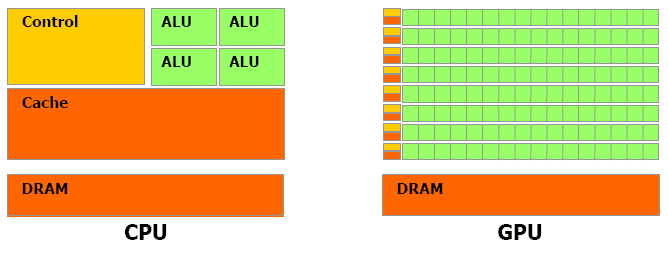
\includegraphics[width=1\linewidth]{compare_paper}}
\caption{Сравнение GPU и CPU}
\label{ris:compare}
\end{figure}
\par 
Многопоточность в графических процессорах также реализована и на аппаратном уровне. На CPU же её задействовать не целесообразно, так как каждое переключение между потоками неизбежно ведёт к значительным временным задержкам продолжительностью в несколько сотен тактов. 
\par 
CPU, будучи универсальным вычислительным устройством, эффективно справляется с целым спектром различных задач, в то время как предназначение графических процессоров гораздо более узконаправленное. В задачах с множественными ветвлениями и переходами графический процессор не столь эффективен как центральный
\par
В связи с особенностями графических процессор они хорошо справляются с задачами, где требуется большое количество параллельных вычислений с большим количеством арифметических операций. Причем элементы данных должны быть независимы (GPU обладает плохим синхронизационным аппаратом) и работа над данными одинакова. 

\section{Технология CUDA}

\cite{cuda_best} \cite{sanders} \cite{kirk} \cite{boreskov}
\par
CUDA (Compute Unified Device Architecture) – это архитектура параллельных вычислений от NVIDIA, позволяющая существенно увеличить вычислительную производительность благодаря использованию GPU (графических процессоров). Для реализации новой вычислительной парадигмы компания NVIDIA изобрела архитектуру параллельных вычислений CUDA, и обеспечивающую необходимую базу разработчикам ПО.
\par
Платформа параллельных вычислений CUDA обеспечивает набор расширений для языков C и С++, позволяющих выражать как параллелизм данных, так и параллелизм задач на уровне мелких и крупных структурных единиц. Всё это является несомненными преимуществами использования CUDA-технологии на ряду с доступностью.
\par
Компания NVIDIA предоставляет показательные примеры кода на CUDA (CUDA Code Samples) в свободной доступе на английском языке и в продаже на русском, а также две платформы Nvidia Nsight Edition для разработчиков в Eclipse и Microsoft Visual Studio. 
\par Перечислим основные характеристики CUDA:
\begin{itemize}
\item[•] Унифицированное программно-аппаратное решение для параллельных вычислений на видеочипах NVIDIA.
\item[•] Большой набор поддерживаемых графических плат (от мобильных до мультичиповых).
\item[•] В качестве языка программирования используется расширенный вариант языка C.
\item[•] Поддерживает взаимодействие с графическими API OpenGL и DirectX.25
\item[•] Имеется поддержка 32- и 64-битных операционных систем: Windows XP, WindowsVista, Linux и MacOSX.
\item[•] Возможность разработки на низком уровне.
\item[•] CUDA обеспечивает доступ к быстрой разделяемой памяти, которая может быть использована для межпоточного взаимодействия.
\end{itemize}
\par
команда разработчиков CUDA  создала набор программных уровней для работы с GPU, которые отображены на Рис.~\ref{ris:cuda_levels}.
\par
\begin{figure}[h]
\center{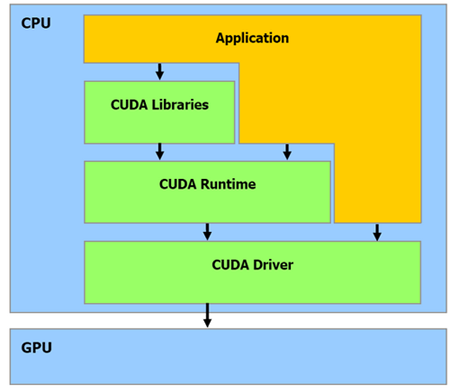
\includegraphics[width=1\linewidth]{cuda_levels}}
\caption{Набор программных уровней для работы с GPU}
\label{ris:cuda_levels}
\end{figure}
\par
Нативный компилятор/отладчик: nvcc/cuda-gdb[linux/mac os], расширение к msvc/TotalView [win].
\par
Если распараллеливать задачу на CPU но следить за потоками нужно самим. При распараллеливании на видеокартах известен только номер нити или блока. А также регулируется количество потоков, которые все исполняют одну последовательность инструкций. Запуск с хоста device-функции - это kernel. У этого ядра существует конфигурация. У нас в распоряжении миллион потоков и внутри device-функции известен только номер потока. Внутри блока нити находятся физически близко и могут делить общую память. Адресация внутри сетки блоков происходит по идентификации блоков и нитей. Может быть несколько измерений (до трёх). Вся забота думать о том, как делать конфигурацию. От этого много чего зависит.
\par
Физический уровень - видеокарта:
\begin{itemize}
\item[•] Streaming Multiprocessor (SM) - “процессор” на видеокарте.
\item[•] Bandwidth – внутренняя пропускная способность. Влияет на копирование dev-dev.
\item[•] PCI-express - шина общения с хостом. Влияет на скорость копирования host-dev.
\end{itemize}
\par
Логический уровень - kernel (ядро) - функция, полностью вычисляющаяся на графическом устройстве:
\begin{itemize}
\item[•] Grid (геометрия сетки блоков нитей) – свойство запуска функции, определяющее количество запускаемых блоков вычислений. Важна как сама геометрия, так и максимизация количества.
\item[•] Thread block (блок нитей) - множество нитей, имеющих общую r/w память, со scope адресации внутри этого блока.
\item[•] Warp – множество одновременно исполняющихся нитей внутри одного cuda core. Имеет особый смысл в случае ветвлений: блок нитей бьется на две части, которые исполняются по сути последовательно. Также понятие warp сильно связано с выравниваниями в памяти.
\end{itemize}
\par
Важно быть аккуратным с ветвлениями. Все нити сначала исполнят одну ветку, потом другую. Такой фокус вследствие SIMD. warp - множество нитей, которые прямо сейчас исполняются. Идеально если warp\_size (ровно 32) совпадает с block\_size. 
\par 
Как можно видеть, CUDA обеспечивает два API:
\begin{itemize}
\item высокоуровневый API: CUDA Runtime API;
\item низкоуровневый API: CUDA Driver API;
\end{itemize}
\par
Каждый вызов фукнции уровня Runtime состоит из более элементарных инструкций уровня Driver API. Стоит помнить, что два API взаимно исключают друг друга. При использовании одного, нельзя использовать функции другого уровня. Driver API сложнее и требует больше знаний о NVIDIA GPU, но при этом он более гибок и предоставляет весь контроль программисту. 
\par 
Потоком в CUDA назвается базовый набор данных, который требуется обработать. В отличие от потоков CPU, переключение контекста между двумя потоками CUDA не является ресурсоёмкой операцией. 32 потока объединяются в один варп - минимальный объём данных, обрабатываемых SIMD-способом в мультипроцессорах CUDA. Также потоки составляют блоки, которые в свою очередь формируют сетки. Если GPU имеет мало ресурсов, то он будет выполнять блоки последовательно. 
\par
\begin{figure}[h]
\center{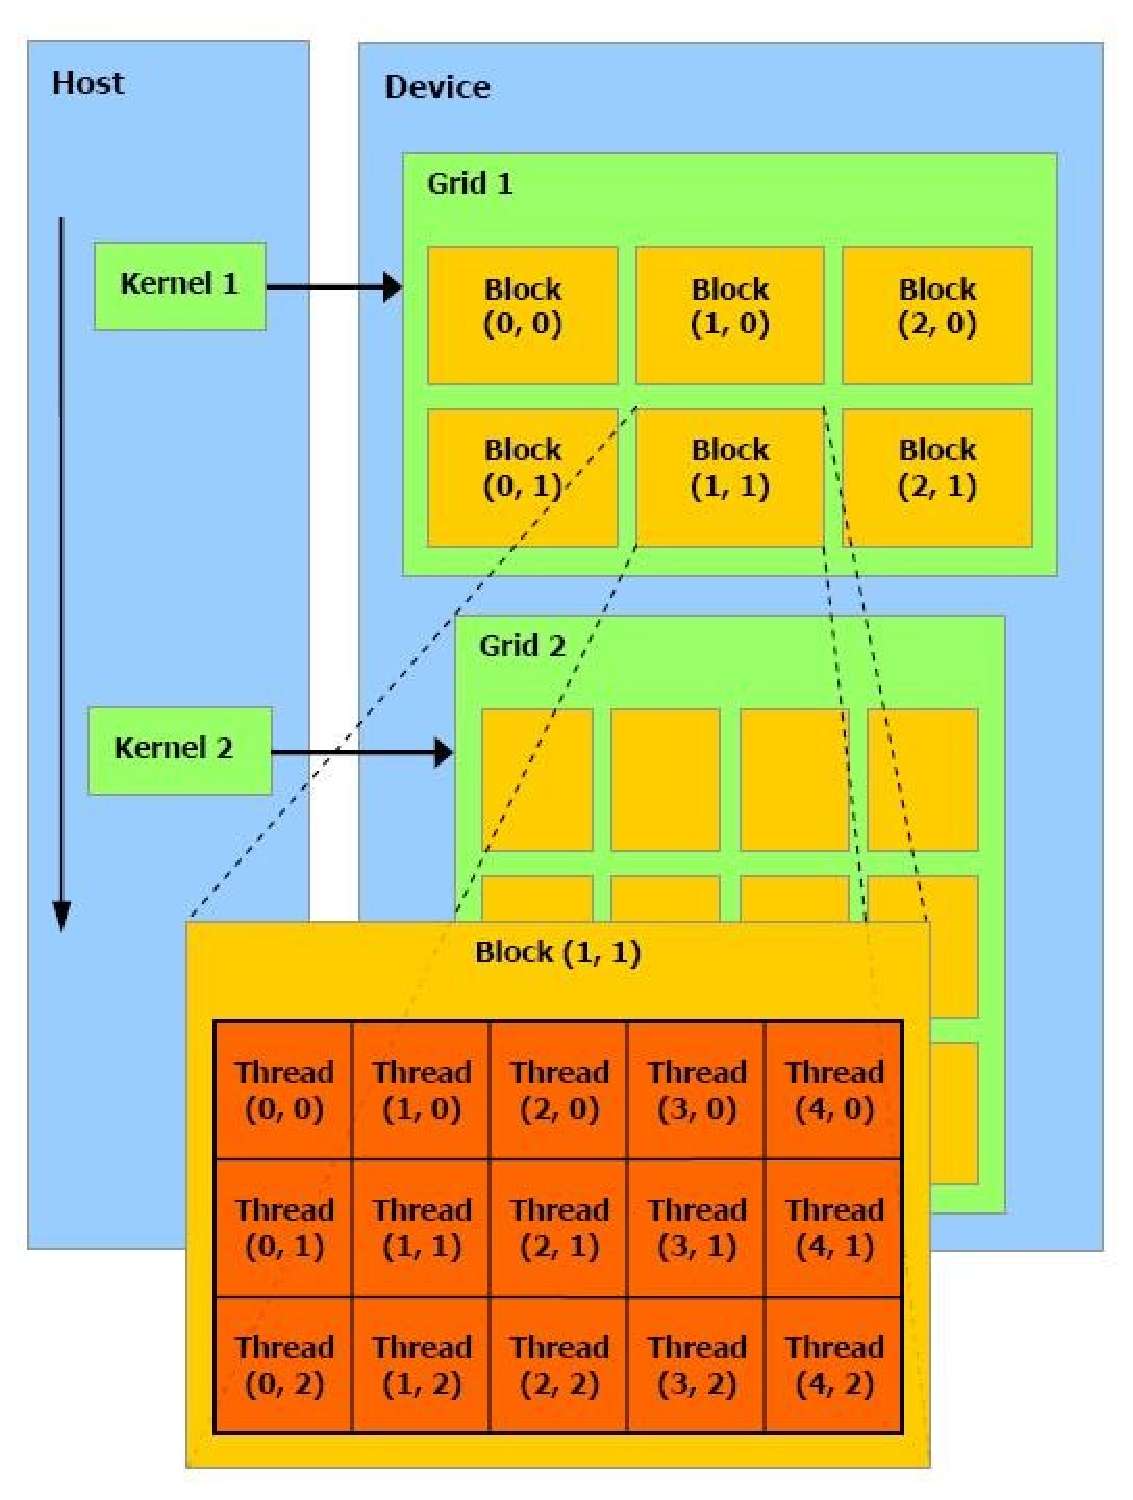
\includegraphics[width=1\linewidth]{thread_block}}
\caption{Конструкция grid}
\label{ris:thread_block}
\end{figure}
\par
\begin{figure}[h]
\center{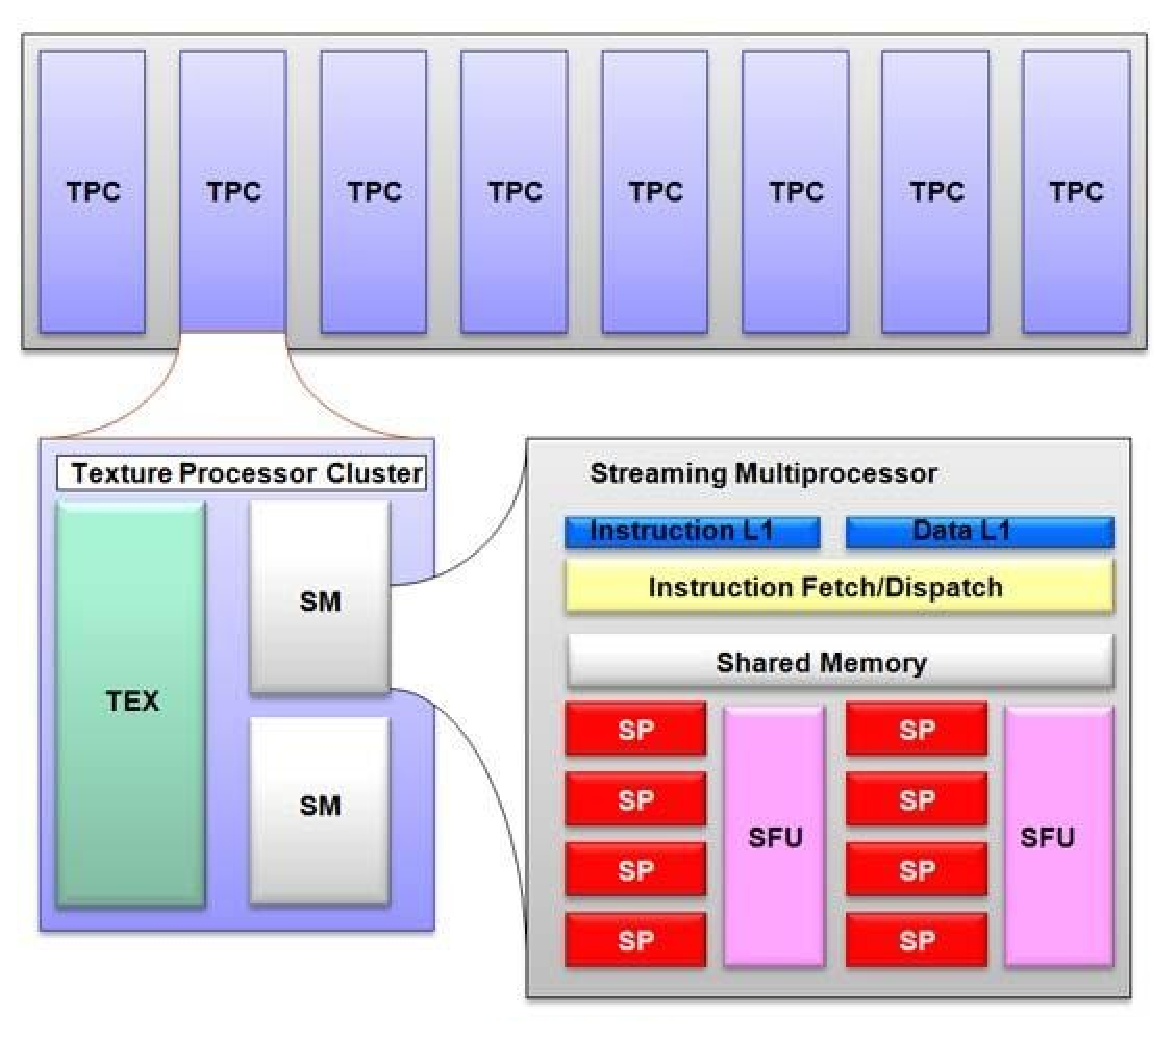
\includegraphics[width=1\linewidth]{tcp}}
\caption{Конструкция TCP и SM}
\label{ris:tcp}
\end{figure}
\par
Видеокарта может содержать несколько (от 2 до 2000) потоковых мультипроцессоров (streaming multiprocessor). Они в свою очередь содержат восемь вычислительных устройств и два суперфункциональных устройства SFU (Super Function Unit), где инструкции выполняются по принципу SIMD, что в данном случае означает применение одной инструкции ко всем потокам в варпе.
\par 
Потоковые мультипроцессоры работают следующим образом: каждый такт начало конвейера выбирает варп, готовый к выполнению, и запускает выполнение инструкции. Чтобы инструкция применилась ко всем 32 потокам в варпе, концу конвейера потребуется четыре такта, но поскольку он работает на удвоенной частоте по сравнению с началом, потребуется только два такта (с точки зрения начала конвейера). Поэтому, чтобы начало конвейера не простаивало такт, а аппаратное обеспечение было максимально загружено, в идеальном случае можно чередовать инструкции каждый такт, классическая инструкция в один такт и инструкция для SFU в другой.
\par 
Мультипроцессор имеет 8192 регистра, которые общие для всех потоков всех блоков, активных на мультипроцессоре. Число активных блоков на мультипроцессор не может превышать восьми, а число активных варпов ограничено 24 (768 потоков).
\par 
Оптимизация программы CUDA, таким образом, состоит в получении оптимального баланса между количеством блоков и их размером. Больше потоков на блок будут полезны для снижения задержек работы с памятью, но и число регистров, доступных на поток, уменьшается. Более того, блок из 512 потоков будет неэффективен, поскольку на мультипроцессоре может быть активным только один блок, что приведёт к потере 256 потоков. Поэтому NVIDIA рекомендует использовать блоки по 128 или 256 потоков, что даёт оптимальный компромисс между снижением задержек и числом регистров для большинства ядер/kernel.
\par 
За формирование и компиляцию ядер отвечает CPU. Видеочип просто
принимает уже скомпилированное ядро и создает его копии для каждого
элемента данных. Каждое из ядер исполняется в своем собственном потоке.

\section{Иерархия памяти}

\begin{figure}[h]
\center{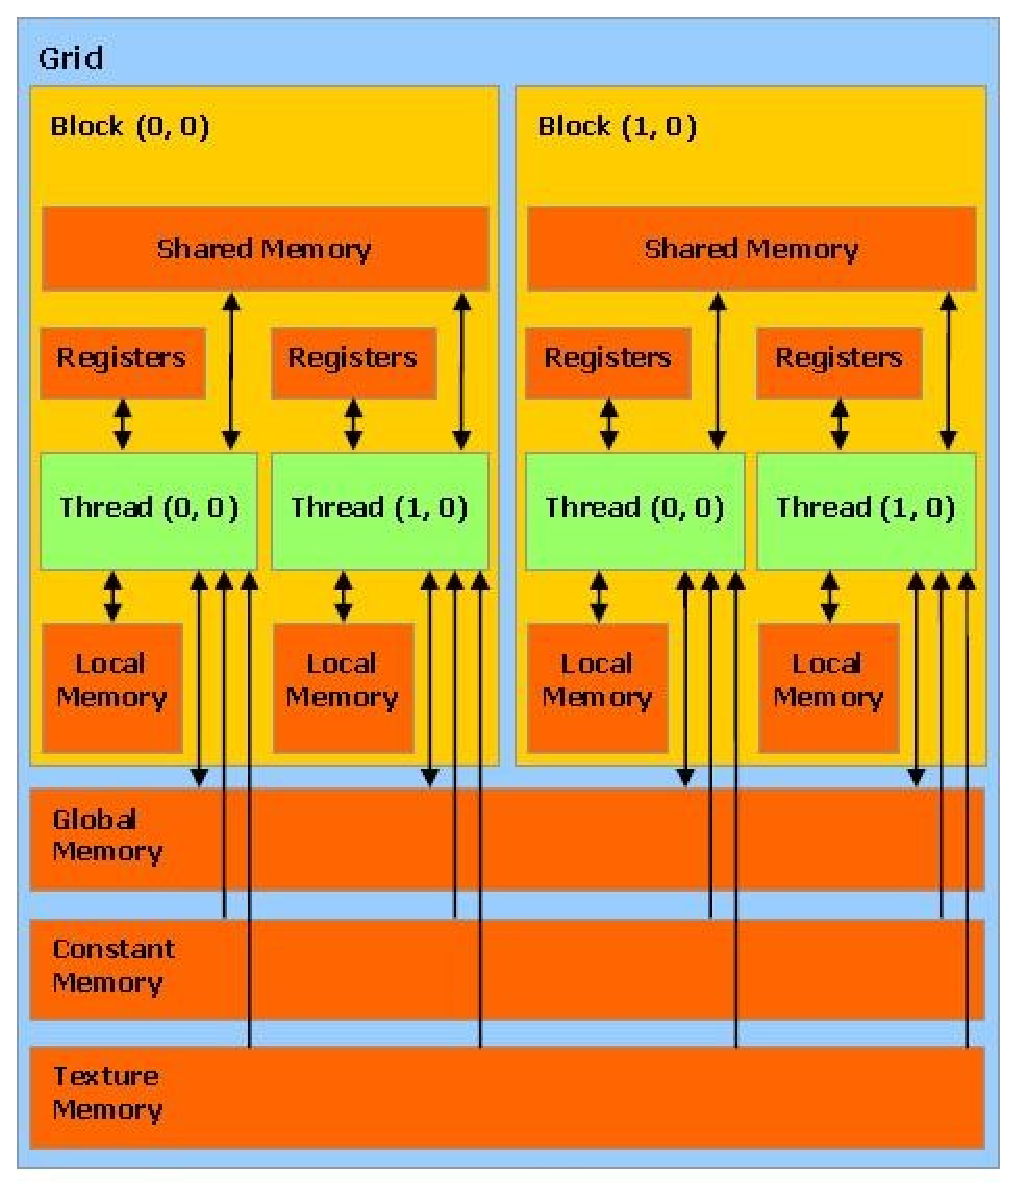
\includegraphics[width=1\linewidth]{mem_hierarchy}}
\caption{Иерархия памяти CUDA}
\label{ris:mem_hierarchy}
\end{figure}
\par 
Вычислительные возможности 2.x
\begin{itemize}
\item[•] Глобальная память (чтение и запись):
  \begin{itemize}
  \item медленная, но может быть кеширована;
  \item последовательное и выровненное чтение по 64 или 128 байт для более быстрого использования. Иначе замедление в 10-100 раз;
  \item плохая параллельная скорость доступа, если пользоваться ей напрямую;
  \item адресация - прямая, по указателям;
  \item видна всей сетке блоков. 
  \end{itemize}
\item[•] Текстурная память (чтение только) - кэш, оптимизированный для двумерного доступа.
  \begin{itemize}
  \item более удобный метод доступа с геометрической точки зрения;
  \item неизменяемая;
  \item кэшируемая.
  \end{itemize}
\item[•] Константная память:
  \begin{itemize}
  \item содержит константы и аргументы функций ядра;
  \item имеет особенные инструкции заполнения;
  \item сравнительно быстрая, но её мало;
  \item видна всей сетке блоков. 
  \end{itemize}
\item[•] Разделяемая память (48кБ на 1 SM):
  \begin{itemize}
  \item быстрая, но подвержена конфликтам в банке памяти;
  \item видна всем нитям внутри блока.
  \end{itemize}
\item[•] Локальная память:
  \begin{itemize}
  \item используется для любых данных, что не влезли в регистровую память;
  \item часть глобальной памяти, поэтому медленная;
  \item автоматическое выравнивание обращений;
  \item видна одной нити.
  \end{itemize}
\item[•] Регистровая память - 32768 32-битных регистра на 1 SM.
\end{itemize}
\par
Константная память целиком кэшируется. Поэтому получается достаточно быстро. У каждой нити свои регистры. Локальные переменные могут попасть как в shared так и global. Блоки обрабатываются конвейерным образом(по 32 штуки?). shared память очень быстрая. аллоцируется статически. 
\par 
Два потока из разных блоков не могут обмениваться информацией между собой во время выполнения. Пользоваться общей памятью не так просто. Общая память всё оправдана за исключением случаев, когда несколько потоков пытаются обратиться к одному банку памяти, вызывая конфликт. 
\par 
Мультипроцессоры также могут обращаться к видеопамяти, но с меньшей пропускной способностью и большими задержками. Поэтому NVIDIA оснастила мультипроцессоры кэшем, хранящим константы и текстуры. 
\par 
Доступ к глобальной памяти имеет свои трудности. Выравнивание доступа к памяти – самый сложный и самый важный аспект в программировании под Nvidia CUDA. Доступ к памяти называется coalesced в том случае, когда массовая операция доступа из одного warp к памяти укладывается в одну транзакцию.
\par 
Для обмена информацией внутри блока между потоками используется разделяемая память (shared memory). РРазделяемая память устроена так, что доступная блоку память разбита на банки памяти с раздельными путями доступа. В случае, если две нити пытаются обратиться в один банк памяти одновременно, возникает “конфликт” и доступ они получают последовательно, а не параллельно. Максимальное количество нитей в блоке, пытающихся обратиться к одному банку, называется “глубиной конфликта доступа”.
\par 
Для интегрированных GPU использование нуль-копируемой памяти всегда даёт выигрыш, потому что эта память в любом случае физически разделяется с CPU. В тех случаях, когда входные и выходные буферы используются ровно один раз, повышение производительности будет наблюдаться и на дискретном GPU.

\section{Программная реализация}
Исследуем последовательный код на CPU на места, наиболее эффективно поддающиеся рапараллеливанию. Для этого обратимся к профайлеру gprof. Ниже приведены результаты исполнения только для функций, исполнение которых составляет больше 0.009 процентов от общего времени.
\\
\begin{tabular}{rrrrrrp{3cm}}
  \% &  cumul. &  self    & &         self  &   total    \\       
 time  & seconds &  seconds  &  calls &  s/call &  s/call & name    \\
 99.67  &   13.21  &  13.21 &   22756 &    0.00 &    0.00 & dualSimplex\\
  0.38  &   13.26  &   0.05  &  22756 &    0.00  &   0.00 & pivotColumn\\
  0.08   &  13.27 &    0.01 & 13986754 &    0.00 &    0.00 &  cmp\\
\end{tabular}
\\
\begin{tabular}{rrrrrrp{3cm}}
  \% &  cumul. &  self  &          &  self  &   total    & \\       
 time  & seconds  & seconds  &  calls & Ks/call & Ks/call &  name  \\  
 84.66 &  1099.81 & 1099.81 &   23063 &    0.00  &   0.00 & multip\\
 15.17 &  1296.83 &  197.02  & 293997  &   0.00  &   0.00 & dualSimplex\\
  0.13 &  1298.58  &   1.75  &  23373  &   0.00  &   0.00 & Matrix::Matrix(int, int, int)\\
  0.07 &  1299.50  &   0.92 &  293999  &   0.00  &   0.00 & pivotColumn\\
  0.02 &  1299.77  &   0.27 & 197223184  &   0.00 &    0.00 & cmp\\
  0.01 &  1299.90  &   0.13  &    308   &  0.00  &   0.00 & Matrix::operator=\\
\end{tabular}
\par
Как видно из таблицы, в первую очередь необходимо оптимизировать произведение матриц. Можно как реализовать собственную функцию произведения матриц, так и воспользоваться уже известной реализацией из библиотеки cuBLAS на GPU, которая есть аналог функции BLAS на CPU. 
\par
BLAS (Basic Linear Algebra Subprograms) - интерфейс, базовые подпрограммы линейной алгебры:
\begin{enumerate}
\item Векторные операции вида $y\Leftarrow\alpha x + y$ - операции скалярного произведения, взятия нормы вектора и др.
\item Операции матрица-вектор вида $y\Leftarrow\alpha Ax + \beta y$, решение $Tx = y$ для $x$ с треугольной матрицей $T$ и др.
\item Операции матрица-матрица вида $C\Leftarrow \alpha AB + \beta C$, решение $B\Leftarrow \alpha T^(-1)B$ для треугольной матрицы $T$ и др.
\end{enumerate}


\subsection{Классы и методы}
Основной класс - это класс матрицы, который называется Matrix. Остановимся на нём подробнее. Он содержит поля:
\begin{itemize}
\item[•] int rows;
\item[•] int cols;
\item[•] double *e;
\item[•] int supply;
\end{itemize}
и методы:
\begin{itemize}
\item[•] Matrix(int rows, int cols, int supply = 0);
\item[•] Matrix(char const *file\_name, int supply = 0);
\item[•] Matrix(Matrix const \&input, int supply = 0);
\item[•] Matrix(Matrix const \&input, unsigned int flag, int supply = 0);
\item[•] ~Matrix();
\item[•] void freeHost();
\item[•] bool print(char const *filename) const;
\item[•] void gcd(int const n);
\item[•] void reinit(int rows, int cols, int supply = 0);
\item[•] void reinit(Matrix const \&matrix1, Matrix const \&matrix2);
\item[•] void pin\_mem ();
\item[•] void unpin\_mem ();
\item[•] Matrix \&operator=(Matrix const \&matrix);
\end{itemize}
\par
Поля rows и cols оответствуют размерам матрицы - количеству строк и колонок соответственно. Поля numer и denom - массивы, хранящие числительное и знаменательное элементов матрицы.
\par
Матрица представлена в виде одномерного массива колонок. Такая реализация выбрана вместо более распространённого представления в виде строк, потому что основные преобразования матрицы происходят при манипуляции колонок. То есть в первую очередь мы нормируем колонку. На следующем шаге мы нормируем ведущую строчку, домножая ведущую колонку на элемент и вычитая из текущей колонки. Что означает, что используемый метод симплекса можно представить в виде манипуляции колонками.
\par 
Последнее поле supply используется при добавлении элементов в матрицу. То есть в этой переменной хранится количество дополнительных свободных ячеек в массивах denom и numer. Это необходимо в алгоритме при добавлении отсечений к матрице.
\par
Перейдём к описанию методов. Первые четыре метода - конструкторы, которые исполбзуют supply как необязательный параметр. Первый конструктор создаёт нулевую матрицу с данным количеством колонок и строк. Второй метод считывает матрицу из текстового файла. В данном файле первые два считанных значения - количество колонок и строк в матрице. Далее попорядку считываются элементы матрицы в виде двух чисел - числитель и знаменатель. Но элементы считываются в построчном виде, по причине того что матрицы в C\\C++ представляются в построчном виде. 
\par
Следующий конструктор принимает на вход матрицу - конструктор копирования. И последний конструктор помимо матрице как обязательный параметр принимает переменную $flag$. Дело в том, что реализация метода с асинхронным копированием использует закреплённую память, так как иначе это может привести ко множеству ошибок. При выделении закрпелённой памяти используется функция cudaHostAlloc, которая в свою очередь использует параметр flags, чтобы специфицировать использование выделяемой памяти.
\par
Деструктор очищает выделенную динамически память. Но нужно запомнить, что при выделении закреплённой памяти нужно очищать выделенную память самостоятельно, для этого используется метод freeHost();
\par
Метод print печатает матрицу в файл, имя которого принимается как входящий аргумент. Метод gcd сокращает элемент матрицы, используя алгоритм Евклида. Оба метода reinit перезаписывают матрицу. Первый метод выделяет памяти ровно столько, сколько требуется, а второй добавляет к существующей матрице дополнительные строчки. 
\par
Методы pin\_mem() и unpin\_mem() закрепляют и открепляют уже выделенную динамически память, которые изначально выделялась незакреплённой.
\par
Для удобства также реализован оператор присваивания.

\subsection{Произведение матриц}
В приведённый алгоритм можно несколько модернизировать при использовании произведения матриц. Так как отсечения добавляются в конец таблицы, то первоначально алгоритм симплекса проходит все те же стадии, что и первоначальная матрица. В таком случае можно сохранить данные преобразования таблицы в некоторую матрицу transformation. Таким образом не придётся много раз выполнять одну и ту же работу. 
\par
Используем всем известный алгоритм произведения матриц строка-столбец. 
 
\subsection{}
\par
Отметим, что обозначенное угловыми скобками ядро также принимает необязательный аргумент stream. Этот запуск ядра выполняется асинхронно, как и две предыдущие операции копирования в память GPU и последующая операция копирования в  память CPU. Строго говоря, не исключено, что мы выйдем из цикла ещё до того, как начнётся копирование памяти или исполнение ядра. Гарантируется лишь, что первая операция копирования, помещённая в поток, завершится до начала второй операции копирования. А вторая операция копирования завершится до начала исполнения ядра, а исполнение ядра закончится до начала третьей операции копирования. То есть, как и было сказано в начале главы, потом ведёт себя как упорядоченная очередь задач для GPU. По выходе из цикла for в очереди ещё могут находиться задания, которые GPU предстоит выполнить.
\par 
Асинхронное копирование имеет смысл, только если поиск пивота происходит на CPU. А эта часть плохо параллелиться, чтобы её производить на гпу, то есть снова асинхронно копировать туда сюда.
\par 
Обработка ошибок требует усовершенствования, так как при возникновении какой-либо программа вызывает аварийное завершение. 
\par 

\chapter{Анализ}
\section{Исследование корректности}
Первоначально при выборке тестов учитывался так же факт того, что важен анализ как эффективности, так и корректности. В работе корректность алгоритма устанавливается при помощи сравнительных тестов в формате DIMACS, которые представляют собой КНФ формулу. Задача выполнимости сводится к нахождению булевого решения (а при добавлении ограничений $x_i <= 1$ и $x_i >= 0$ к нахождению целочисленного решения) некоторой системы линейных уравнений, составленных на основании КНФ формулы. Таким образом мы проверяем корректность алгоритма, зная выполнима формула или нет.
\par

\section{Исследование эффективности}
Симплекс-метод широко используется и хорошо работает на практике: многочисленные эксперименты подтверждают почти линейную по числу переменных оценку числа итераций. Однако можно показать, что на специальных примерах симплекс-метод (при некотором правиле выбора направляющего столбца и направляющей строки) работает экспоненциально долго. Первыми такой пример предложили Виктор Кли и Джордж Джеймс Минти в 1972 г.:
$$\max(2^{n-1}x_1 + 2^{n-2}x_2 + 2x_{n-1} + x_n)$$
$$\left\{ \begin{tabular}{lcr} 
$x_1$ & $\leq$ & 5, \\
$4x_1 + x_2$ & $\leq$ & 25, \\
$8x_1 + 4x_2 + x_3$ & $\leq$ & 125, \\
\multicolumn{3}{l}{\ldots\ldots\ldots\ldots\ldots\ldots\ldots\ldots\ldots\ldots\ldots\ldots\ldots\ldots\ldots\ldots\ldots}\\
$2^nx_1 + 2^{n-1}x_2 + 2^{n-2}x_3 + ... + 4x_{n-1} + x_n$ & $\leq$ & $5^n$,
\end{tabular}\right.$$
В этом случае используемый в работе симплекс-метод выполнит $2^n-1$ итераций. Хотя для существуют другие правила выбора pivot\_row и pivot\_col, которые решают задачу за константное число операций, для них также существуют задачи, на которых алгоритм работает экспоненциально.
\par
С другой стороны, алгоритмы решающие задачу линейного программирования за полиномиальное время существуют и, следовательно, она принадлежит классу $P$. Этот вопрос был решён в 1979 г. Л.Г.Хачияном, российским математиком. Он использовал метод эллипсоидов, разработанный для задач нелинейного программирования Н.З.Шором, Д.Б.Юдиным и А.С.Немировским. Хотя алгоритм Хачияна и его модификафии эффективны с теоретической точки зрени, практически конкурировать с симплекс-методом она, по крайней мере, пока, не могут. 
\par 
Наложив ограничение целочисленности на все или часть переменных, мы получаем задачу целочисленного линейного программирования, которая оказывается намного более трудной, чем задача линейного программирования. Задача о совместности условий задачи целочисленного программирования принадлежит классу $NP$-полных. 
\par
Упражнения из учебника (с.146 Шевченко Золотых) \\
Алгоритм Branch-and-Bound экспоненциально ($2^t$ итераций) зависит от длины записи коэффициентов задачи целочисленного линейного программирования:
$$\max x_1$$
$$\left\{ \begin{tabular}{l}
$(2^t + 1)x_1=2^tx_2,$ \\
$0\leq x_2 \leq 2^t,$ \\
$x_1,x_2\in\mathbb{Z}.$
\end{tabular}\right.$$
\par
Для установления несовместности условий задачи целочисленного линейного программирования $$\max(x_1 + x_2 + ... + x_n)$$
$$\left\{\begin{tabular}{l}
$2x_1 + 2x_2 + ... + 2x_n = n$ \\
$x_j\in\mathbb{Z}, (j=1,2,..,n)$
\end{tabular}\right.$$
где $n$ - нечётно, Branch-and-Cut требует $2^{\frac{n+1}{2}}$ итераций. Таким образом, трудоёмкость зависит от числа переменных. 
\par
Мерой исследования эффективности на практике было выбрано время. Сводка результатов приведена ниже в таблице:
\begin{tabbing}
test name mmmmmm \= rows \= cols \= iters \= CPU, ms \= dev, ms \= async, ms \= sync, ms \kill
test name \> rows \> cols \> iters \> CPU, ms \> dev, ms \> async, ms \> sync, ms \\
uf20-01.cnf	\> 132	\> 21	\> 27	\> 5	\> 90	\> 6	\> 9 \\
uf20-03.cnf	\> 132	\> 21	\> 60	\> 10	\> 105	\> 8	\> 9 \\
uf20-09.cnf	\> 132	\> 21	\> 77	\> 16	\> 131	\> 11	\> 14 \\
hole6.cnf	\> 190	\> 43	\> 22	\> 4	\> 98	\> 6	\> 6 \\
uuf50-01.cnf	\> 304	\> 51	\> 456	\> 327	\> 566	\> 74	\> 285 \\
uuf50-03.cnf	\> 319	\> 51	\> 172	\> 94	\> 239	\> 31	\> 98 \\
uf50-04.cnf	\> 319	\> 51	\> 207	\> 125	\> 282	\> 38	\> 122 \\
uuf50-02.cnf	\> 319	\> 51	\> 265	\> 180	\> 374	\> 52	\> 167 \\
uf50-01.cnf	\> 319	\> 51	\> 317	\> 214	\> 407	\> 53	\> 191 \\
uf50-05.cnf	\> 319	\> 51	\> 465	\> 360	\> 643	\> 80	\> 338 \\
hole8.cnf	\> 368	\> 73	\> 29	\> 17	\> 103	\> 12	\> 20 \\
uuf75-01.cnf	\> 450	\> 76	\> 35	\> 1037	\> 1203	\> 208	\> 960 \\
uf75-08.cnf	\> 467	\> 6	\> 1181	\> 1861	\> 1912	\> 342	\> 1720 \\
uuf75-02.cnf	\> 469	\> 76	\> 909	\> 1606	\> 1592	\> 276	\> 1505 \\
uuf75-04.cnf	\> 470	\> 76	\> 1354	\> 2264	\> 2239	\> 401	\> 2106 \\
uf75-01.cnf	\> 476	\> 76	\> 511	\> 773	\> 805	\> 151	\> 729 \\
uf75-04.cnf	\> 476	\> 76	\> 782	\> 1429	\> 1443	\> 242	\> 1328 \\
uf75-02.cnf	\> 476	\> 76	\> 911	\> 1880	\> 1803	\> 285	\> 1620 \\
flat30-100.cnf	\> 481	\> 91	\> 61	\> 55	\> 121	\> 22	\> 54 \\
BMS\_k3\_n100\_m4...	\> 487	\> 101	\> 908	\> 1642	\> 1526	\> 315	\> 1384 \\
hole9.cnf	\> 541	\> 91	\> 45	\> 49	\> 177	\> 20	\> 49 \\
CBS\_k3\_n100\_m4...	\> 612	\> 101	\> 1784	\> 5062	\> 5285	\> 807	\> 4689 \\
RTI\_k3\_n100\_m42...	\> 619	\> 101	\> 1628	\> 4911	\> 4860	\> 738	\> 4568 \\
uuf100-01.cnf	\> 622	\> 101	\> 1553	\> 4509	\> 4305	\> 706	\> 4183 \\
uf100-01.cnf	\> 631	\> 101	\> 2055	\> 6233	\> 5968	\> 934	\> 5756 \\
CBS\_k3\_n100\_m4...	\> 650	\> 101	\> 1150	\> 2855	\> 2681	\> 524	\> 2621 \\
hole10.cnf	\> 626	\> 111	\> 44	\> 65	\> 171	\> 22	\> 61 \\
uuf125-01.cnf	\> 763	\> 126	\> 3275	\> 14425	\> 11439	\> 1985	\> 13429 \\
uf125-01.cnf	\> 789	\> 126	\> 3879	\> 19345	\> 17822	\> 2879	\> 18399 \\
flat50-100.cnf	\> 846	\> 151	\> 98	\> 253	\> 218	\> 74	\> 238 \\
uuf150-01.cnf	\> 913	\> 151	\> 3320	\> 20960	\> 17169	\> 2902	\> 20192 \\
uuf175-01.cnf	\> 1002	\> 176	\> 3235	\> 21859	\> 16009	\> 3040	\> 20210
\end{tabbing}
\par
Тесты в таблице отсортированы по количеству ячеек в матрице, т.е. $rows * cols$. Значения в колонке таковы: 
\begin{itemize}
\item[•] имя тестового файла;
\item[•] количество строк в матрице, т.е. размер колонки;
\item[•] количество колонок в матрице, т.е. размер строки;
\item[•] количество итераций в алгоритме симплекс-метода (одинаковое для всех реализаций);
\item[•] время, потраченное на симплекс-метод, реализованный абсолютно на CPU;
\item[•] время, потраченное на симплекс-метод, реализованный абсолютно на GPU;
\item[•] время, потраченное на симплекс-метод, реализованный частично на GPU и CPU при использовании асинхронного копирования из одной памяти в другую;
\item[•] время, потраченное на симплекс-метод, реализованный частично на GPU и CPU при использовании синхронного копирования из одной памяти в другую;
\end{itemize}
\par
Исходя из полученных данных, считаю целесообразным из всех реализаций симплекс-метода при помощи GPU, использовать подход,частично использующий GPU и CPU и реализованный с использованием асинхронного копирования. Далее уделим внимание этой реализации алгоритма. 

\section{Подробное исследование эффективности выбранного метода}
Было проведено более подробное исследование эффективности выбранного метода. Оно состояло из трёх этапов:
\begin{enumerate}
\item[1.] Фиксируем количество ограничений и меняем количество переменных.
\item[2.] Фиксируем количество переменных и меняем количество ограничений.
\item[3.] Фиксируем отношение ограничений к переменным и меняем число переменных. 
\end{enumerate}
\par


\section{Теоретический анализ выбранного метода}
Определим понятие масштабируемости. Масштабируемость (англ. scalability) означает способность системы, сети или процесса справляться с увеличением рабочей нагрузки (увеличивать свою производительность) при добавлении ресурсов (обычно аппаратных). 
\par
Существует два показателя масштабируемости: сильная и слабая. Сильная масштабируемость показывает, как меняется время решения задачи с увеличением количества процессоров (или вычислительных узлов) при неизменном общем объёме задачи. Сильная масштабируемость определяется законом Амдала. Слабая масштабируемость показывает, как меняется время решения задачи с увеличением количества процессоров (узлов) при неизменном объёме задачи для одного процессора (или узла), и определяется законом Густафсона.
\par
Закон Амдала может определить верхнюю грань ожидаемого ускорения за счёт увеличения количества процессоров с фиксированным объёмом задачи. Он выглядит как:
$$S=\frac{1}{\left(1-P\right)+\frac{P}{N}}$$, где $S$ - ускорение выполнения программы, которое по определению равно отношению времени вычисления программы на одном процессоре ко времени вычисления на нескольких процессорах, $P$ - это доля исполнения части кода, которая может быть распараллелена, от общего времени исполнения всего кода, а $N$ - это количество процессоров, на которые может быть распараллелена исследуемая часть кода. Из формулы очевидно следует, что чем больше $N$, тем больше ускорение.
\par 
Исключим $N$ из формулы, устремив его к бесконечности. Отсюда $$S = \frac{1}{1-P}$$. В большинстве случаев программы не демонстрируют идеального ускорения. Но закон Амдала указывает на то, что для достижения ускорения стоит увеличивать распараллеливаемую часть. Если она маленькая, то программа не параллелизуема.
\par
Закон Густафсона измеряет ускорение программы при увеличении количества процессоров и неизменном размере задачи на один процессор, т.е. объём задачи увеличивается пропорционально количеству процессоров. Он определяется формулой: $$S=N+(1-P(1-N)$$, где $P$ и $N$ принимают те же обозначения, что в формуле Амдала. 
\par
Цель такого подхода - за заданное время выполнить максимальный объем вычислений.
\par


\chapter{Результаты и выводы}
Привести здесь отзывы профайлера.
\par 
Вывод должен отражать коэффициент распараллеливаемости. То есть без учета того, что GPU как правило медленнее CPU, оцениваем отношение шагов. 

\section{Дальнейшее исследование}

\bibliographystyle{utf8gost705u}
\bibliography{biblio} 

\end{document}
\grid
\grid
